\xiti
\begin{xiaotis}

\xiaoti{}%
\begin{xiaoxiaotis}%
    \xxt[\xxtsep]{要在墙上钉稳一根横木条,至少要钉几个钉?为什么?}

    \xxt{在教室里要将一行桌子排齐可以用什么方法? 你能说出这种方法的道理吗?}

    \xxt{将甲、乙两尺如图那样拼在一起, 如果甲尺经校定为直的,那么乙尺可能是直的吗?为什么?}

\end{xiaoxiaotis}

\begin{figure}[htbp]
    \centering
    \begin{minipage}[b]{7cm}
        \centering
        \begin{tikzpicture}
	\tkzDefPoints{0/0/A, 4/0/B,  0/0.5/A1,  4/0.5/B1,  0/-0.5/A2,  4/-0.5/B2, 2/10/O}
	\tkzDrawPolygon(A,B,B1,A1)
	\tkzLabelSegment[right=1em](B,B1){甲}

	\tkzDrawArc(O,A)(B)
	\tkzDrawArc(O,A2)(B2)
	\tkzDrawSegments(A,A2  B,B2)
	\tkzLabelSegment[right=1em](B,B2){乙}
\end{tikzpicture}


        \caption*{(第 1 题)}
    \end{minipage}
    \qquad
    \begin{minipage}[b]{7cm}
        \centering
        \begin{tikzpicture}
	\tkzDefPoints{0/0/B, 0.4/1/A, 1.5/0.5/C}
	\tkzDrawPoints[fill=black](A,B,C)
	\tkzLabelPoints[above](A)
	\tkzLabelPoints[below](B)
	\tkzLabelPoints[right](C)
\end{tikzpicture}

        \caption*{(第 3 题)}
    \end{minipage}
\end{figure}

\xiaoti{当点 $A$ 在直线 $BC$ 上时, 过三点 $A$、$B$、$C$ 的直线有几条? 当点 $A$ 不在直线 $BC$ 上时,过这三点可以画一条直线吗?}

\xiaoti{已知点 $A$、$B$、$C$ 不在同一条直线上,它们的位置如图。(1)画线段 $AB$; (2) 画射线 $AC$; (3)画直线 $BC$。}

\xiaoti{在直线 $AB$ 上分别以 $O$、$D$、$E$ 为端点的射线典有几条?怎样表示它们?}

\begin{figure}[htbp]
    \centering
    \begin{minipage}[b]{7cm}
        \centering
        \begin{tikzpicture}
	\tkzDefPoints{0/0/A, 0.8/0/D, 2/0/O,  3/0/E, 4/0/B}
	\tkzDrawSegment(A,B)
	\tkzDrawPoints[fill=black](D,O,E)
	\tkzLabelPoints[below](A,D,O,E,B)
\end{tikzpicture}


        \caption*{(第 4 题)}
    \end{minipage}
    \qquad
    \begin{minipage}[b]{7cm}
        \centering
        \begin{tikzpicture}[scale=0.6]
	\tkzDefPoints{0/0/A, 7/0/B, 7/3.5/C,  0/3.5/D}
	\tkzDrawPolygon(A,B,C,D)
	\tkzLabelPoints[above](D,C)
	\tkzLabelPoints[below](A,B)
\end{tikzpicture}


        \caption*{(第 5 题)}
    \end{minipage}
\end{figure}

\xiaoti{用两脚规和刻度尺量出图中线段 $AB$、$BC$、$CD$、$DA$ 的长度(精确到 l mm), 并汁算:}
\begin{xiaoxiaotis}

    \xxt{$AB + BC + CD + DA$;}

    \xxt{$2(AB + BC)$。}

\end{xiaoxiaotis}


\xiaoti{如图,在直接测 $l$ 的长度不方便时,可以先量得 $h$、$m$、$n$ 的长,再计算 $l$ 的长。}
\begin{xiaoxiaotis}

    \xxt{用 $h$、$m$、$n$ 的代数式表示 $l$;}

    \xxt{已知 $h = 31$ mm,$n = 5$ mm, $m = 8$ mm, 计算 $l$ 的长度。}

\end{xiaoxiaotis}


\begin{figure}[htbp]
    \centering
    \begin{minipage}[b]{5cm}
        \centering
        \begin{tikzpicture}
	\pgfmathsetmacro{\h}{3.1}
	\pgfmathsetmacro{\n}{0.5}
	\pgfmathsetmacro{\m}{0.8}
	\pgfmathsetmacro{\l}{1.8}
	\pgfmathsetmacro{\x}{0.8}
	\pgfmathsetmacro{\y}{2.8}
	\tkzDefPoints{0/0/A, \n/0/B, \n/\x/C,  \n+\l/\x+\x/D, \n+\l/\x/E,  \h/\x/F,  \h/\y/G,  0/\y/H}
	\tkzDrawPolygon[thick](A,...,H)
	\tkzDefPoints{\n+\l/0/E', \h/0/F'}

	%\tkzDrawSegment[dim={$n$,-10pt,}](A,B)
	\tkzDefPoints{-0.3/-0.35/x1, 0/-0.35/x2}
	\tkzDrawSegment[-latex](x1,x2)
	\tkzLabelSegment[below=5pt](A,B){$n$}

	\tkzDrawSegment[dim={$l$,-10pt,}](B,E')
	\tkzDrawSegment[dim={$m$,-10pt,}](E',F')  \tkzDrawSegments(E,E'  F,F')
	\tkzDrawSegment[dim={$h$,-20pt,}](A,F')
\end{tikzpicture}

        \caption*{(第 6 题)}
    \end{minipage}
    \qquad
    \begin{minipage}[b]{9cm}
        \centering
        \begin{tikzpicture}[scale=0.8]
	\pgfmathsetmacro{\x}{0.6}
	\pgfmathsetmacro{\y}{5.1}
	\pgfmathsetmacro{\z}{1.9}
	\pgfmathsetmacro{\a}{\x+\y+\z}
	\pgfmathsetmacro{\b}{2.6}
	\pgfmathsetmacro{\bb}{\b/2}
	\pgfmathsetmacro{\d}{0.2}
	\pgfmathsetmacro{\m}{0.3}
	\pgfmathsetmacro{\n}{0.2}

	\tkzDefPoints{0/0/A1,  0/\b/A2,
				 \x/0/B1,    \x/\b/B2,     \x/\m/B3,        \x/\b-\m/B4,
				 \x+\y/\m/C1, \x+\y/\b-\m/C2,  \x+\y+\d/\m+\n/C3, \x+\y+\d/\b-\m-\n/C4,
				 \a/\m+\n+\n/D1, \a/\b-\m-\n-\n/D2,  \a-\d/\m+\n/D3, \a-\d/\b-\m-\n/D4,
				 0/\bb/O1, \a/\bb/O2}
	\tkzDrawPolygon[thick](A1,B1,B2,A2)
	\tkzDrawPolygon[thick](B3,C1,C2,B4)
	\tkzDrawPolygon[thick](C1,C3,D3,D4,C4,C2)
	\tkzDrawPolygon[thick](D1,D2,D4,D3)
	\tkzDrawLine[dash dot,add=0.1 and 0.2](O1,O2)

	\tkzDefPoints{0/-1/A, \x/-1/B, \x+\y/-1/C, \a/-1/D}

	\tkzDrawLine[add=0.1 and 0.2](A,D)
	\tkzDrawSegments(A1,A  B1,B  C1,C D1,D)

	%\tkzDrawSegment[dim={$x$,10pt,}](A,B)
	\tkzDefPoints{-0.4/-0.6/x1, 0/-0.6/x2}
	\tkzDrawSegment[-latex](x1,x2)
	\tkzLabelSegment[above=5pt](A,B){$x$}

	\tkzDrawSegment[dim={$y$,10pt,}](B,C)
	\tkzLabelPoints[below](A,B,C,D)
\end{tikzpicture}


        \caption*{(第 7 题)}
    \end{minipage}
\end{figure}


\xiaoti{如图,已知 $AD = 76$ mm、$BD = 70$ mm、 $CD = 19$ mm,求 $AB$ 的长 $x$ 和 $BC$ 的长 $y$。}


\xiaoti{已知线段 $AB$, 在 $AB$ 的延长线上取一点 $C$, 使 $BC = AB$, 再在 $BA$ 的延长线上取一点 $D$, 使 $DA = 2AB$。
    (1)线段 $AC$ 等于线段 $AB$ 的几倍? (2) 线段 $AB$ 等于线段 $DB$ 的几分之几? (3〕线段 $DB$ 等于线段 $DC$ 的几分之几?
}


\xiaoti{已知线段 $a$、$b$、$c \; (a > b)$,用直尺和圆规画一条线段,使它等于 $a - b + c$。}

\xiaoti{已知线段 $a$、$b \; (a > b)$, 用直尺和圆规画一条线段,使它等于
    (1) $a + 3b$; (2) $2a — b$; (3) $2(a - b)$。
}


\xiaoti{根据图形填空:}
\begin{xiaoxiaotis}

    \xxt{$AC = \ewkh + BC$;}

    \xxt{$CD = AD - \ewkh$;}

    \xxt{$AB + BC = \ewkh - CD$;}

    \xxt{如果 $AB = CD$, $AC$ 与 $BD$ 相等吗? 如果 $AC =BD$, $AB$ 与 $CD$ 相等吗?}

\end{xiaoxiaotis}

\begin{figure}[htbp]
    \centering
    \begin{minipage}[b]{5cm}
        \centering
        \begin{tikzpicture}
	\tkzDefPoints{0/0/A, 1/0/B, 3/0/C, 4/0/D}
	\tkzDrawSegments[xianduan={below=0pt}](A,B  B,C  C,D)
	\tkzLabelPoints[above=0.3em](A,B,C,D)
\end{tikzpicture}


        \caption*{(第 11 题)}
    \end{minipage}
    \qquad
    \begin{minipage}[b]{4cm}
        \centering
        \begin{tikzpicture}
	\tkzDefPoints{0/0/A, 1.5/0/M, 3/0/B}
	\tkzDrawSegments[xianduan={below=0pt}](A,M  M,B)
	\tkzLabelPoints[above=0.3em](A,M,B)
\end{tikzpicture}


        \caption*{(第 12 题)}
    \end{minipage}
    \qquad
    \begin{minipage}[b]{4cm}
        \centering
        \begin{tikzpicture}
	\tkzDefPoints{0/0/A, 0.9/0/C, 3/0/B}
	\tkzDrawSegments[xianduan={below=0pt}](A,C  C,B)
	\tkzLabelPoints[above=0.3em](A,C,B)
\end{tikzpicture}


        \caption*{(第 13 题)}
    \end{minipage}
\end{figure}

\begin{enhancedline}
\xiaoti{点 $M$ 是线段 $AB$ 的中点, 根据图形填空:}
\begin{xiaoxiaotis}

    \xxt{$AM = \ewkh$;}

    \xxt{$BM = \exdfrac{1}{2}\;\ewkh$;}

    \xxt{$AB = 2\;\ewkh - 2\;\ewkh$。}

\end{xiaoxiaotis}

\xiaoti{已知线段 $AB$ 与它上面的一点 $C$, 画线段 $AC$ 的中点 $D$、线段 $BC$ 的中点 $E$。 那么 $DE = \exdfrac{1}{2} AB$ 吗?}
\end{enhancedline}

\end{xiaotis}

